% This file was created with tikzplotlib v0.10.1.
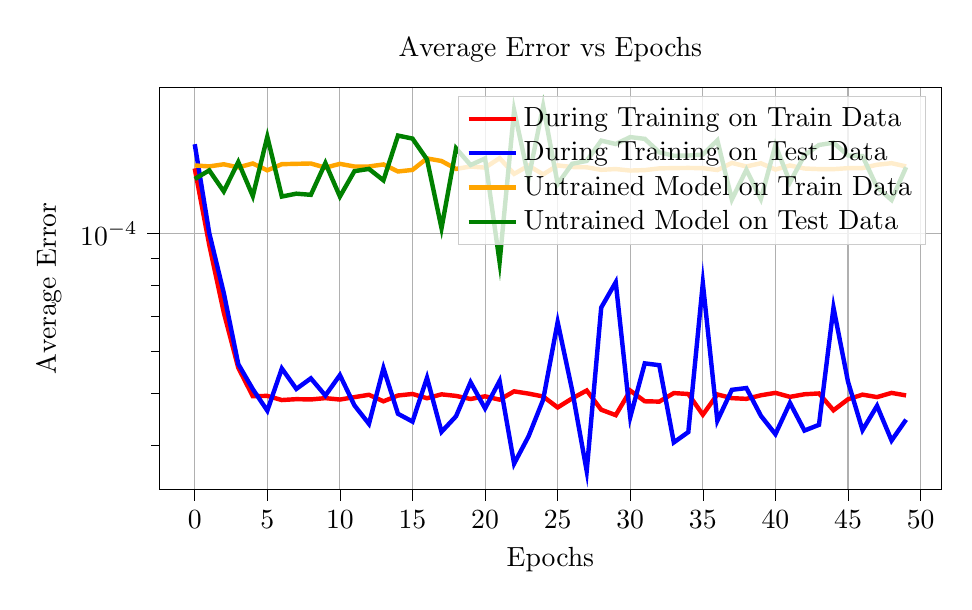
\begin{tikzpicture}

  \definecolor{darkgray176}{RGB}{176,176,176}
  \definecolor{green}{RGB}{0,128,0}
  \definecolor{lightgray204}{RGB}{204,204,204}
  \definecolor{orange}{RGB}{255,165,0}
  
  \begin{axis}[
    width = 0.95\textwidth,
    height = 19em,
  legend cell align={left},
  legend style={
    fill opacity=0.8,
    draw opacity=1,
    text opacity=1,
    % at={(0.91,0.5)},
    % anchor=east,
    draw=lightgray204
  },
  % log basis y={10},
  tick align=outside,
  tick pos=left,
  title={Average Error vs Epochs},
  x grid style={darkgray176},
  xlabel={Epochs},
  xmajorgrids,
  xmin=-2.45, xmax=51.45,
  xtick style={color=black},
  y grid style={darkgray176},
  ylabel={Average Error},
  ymajorgrids,
  ymin=3.30722135247185e-05, ymax=0.000188104234714924,
  ymode=log,
  ytick style={color=black},
  ytick={1e-06,1e-05,0.0001,0.001,0.01},
  yticklabels={
    \(\displaystyle {10^{-6}}\),
    \(\displaystyle {10^{-5}}\),
    \(\displaystyle {10^{-4}}\),
    \(\displaystyle {10^{-3}}\),
    \(\displaystyle {10^{-2}}\)
  }
  ]
  \addplot [ultra thick, red]
  table {%
  0 0.000132722096168436
  1 9.52958143898286e-05
  2 7.11312095518224e-05
  3 5.59525251446757e-05
  4 4.94734194944613e-05
  5 4.95356325700413e-05
  6 4.86540520796552e-05
  7 4.88426849187817e-05
  8 4.87789220642298e-05
  9 4.90620986965951e-05
  10 4.87564029754139e-05
  11 4.92705366923474e-05
  12 4.97732726216782e-05
  13 4.83878284285311e-05
  14 4.96224929520395e-05
  15 4.99510824738536e-05
  16 4.90340717078652e-05
  17 4.98722329211887e-05
  18 4.95317617605906e-05
  19 4.88754849357065e-05
  20 4.94462146889418e-05
  21 4.87317229271866e-05
  22 5.05235257151071e-05
  23 5.0024245865643e-05
  24 4.94094638270326e-05
  25 4.71192179247737e-05
  26 4.90080456074793e-05
  27 5.07079239469022e-05
  28 4.66571473225486e-05
  29 4.55734552815557e-05
  30 5.06827636854723e-05
  31 4.83968869957607e-05
  32 4.83256881125271e-05
  33 5.0144979468314e-05
  34 4.99464476888534e-05
  35 4.56594752904493e-05
  36 4.98443841934204e-05
  37 4.90569836983923e-05
  38 4.89077756355982e-05
  39 4.96737193316221e-05
  40 5.01869035360869e-05
  41 4.93312109028921e-05
  42 4.98860681545921e-05
  43 5.00653732160572e-05
  44 4.65431585325859e-05
  45 4.88188707095105e-05
  46 4.98049921588972e-05
  47 4.92811013828032e-05
  48 5.01822796650231e-05
  49 4.96389002364594e-05
  };
  \addlegendentry{During Training on Train Data}
  \addplot [ultra thick, blue]
  table {%
  0 0.000147356346133165
  1 0.000100276833109092
  2 7.74033032939769e-05
  3 5.68429713894147e-05
  4 5.10137870151084e-05
  5 4.64688382635359e-05
  6 5.57806524739135e-05
  7 5.1057828386547e-05
  8 5.34521313966252e-05
  9 4.96142783958931e-05
  10 5.42103043699171e-05
  11 4.7545585402986e-05
  12 4.38857059634756e-05
  13 5.58492865820881e-05
  14 4.58449612779077e-05
  15 4.43196513515431e-05
  16 5.35876279172953e-05
  17 4.23945093643852e-05
  18 4.53545399068389e-05
  19 5.25535251654219e-05
  20 4.69236656499561e-05
  21 5.28460477653425e-05
  22 3.69406589015853e-05
  23 4.16071488871239e-05
  24 4.87198121845722e-05
  25 6.8199158704374e-05
  26 5.0729689974105e-05
  27 3.57913850166369e-05
  28 7.26350262993947e-05
  29 8.1043537647929e-05
  30 4.51905725640245e-05
  31 5.70314368815161e-05
  32 5.65893242310267e-05
  33 4.04946149501484e-05
  34 4.23562341893557e-05
  35 8.07066462584771e-05
  36 4.44882716692518e-05
  37 5.08558587171137e-05
  38 5.12504157086369e-05
  39 4.54418550361879e-05
  40 4.19671923737042e-05
  41 4.80627386423294e-05
  42 4.26279038947541e-05
  43 4.37011694884859e-05
  44 7.25988211343065e-05
  45 5.26790354342666e-05
  46 4.27131417382043e-05
  47 4.74478620162699e-05
  48 4.08320811402518e-05
  49 4.46896556240972e-05
  };
  \addlegendentry{During Training on Test Data}
  \addplot [ultra thick, orange]
  table {%
  0 0.000134415182401426
  1 0.000133859735797159
  2 0.000135096372105181
  3 0.000133315537823364
  4 0.000135558802867308
  5 0.000131604872876778
  6 0.000135166221298277
  7 0.000135371694341302
  8 0.00013555760961026
  9 0.000133147303131409
  10 0.000135355425300077
  11 0.000133816851302981
  12 0.00013382603356149
  13 0.000135015754494816
  14 0.000130949250888079
  15 0.000131850087200291
  16 0.000138567527756095
  17 0.000137042501592077
  18 0.000132412038510665
  19 0.000133806184749119
  20 0.00013315056276042
  21 0.000138728239107877
  22 0.000129598542116582
  23 0.000134296817122959
  24 0.000129316467791796
  25 0.000134426998556592
  26 0.000133511028252542
  27 0.000133338689920492
  28 0.000131890992633998
  29 0.000132342014694586
  30 0.000131475171656348
  31 0.000131742417579517
  32 0.000132709450554103
  33 0.000132882501929998
  34 0.000132975561427884
  35 0.0001328465732513
  36 0.000131782973767258
  37 0.000135892565594986
  38 0.000133842084323987
  39 0.000135688576847315
  40 0.000132072207634337
  41 0.000134420246467926
  42 0.000132650457089767
  43 0.000132311062770896
  44 0.000132282293634489
  45 0.000132839733851142
  46 0.00013292086077854
  47 0.00013482163194567
  48 0.000135752008645795
  49 0.000133861845824867
  };
  \addlegendentry{Untrained Model on Train Data}
  \addplot [ultra thick, green]
  table {%
  0 0.00012677519407589
  1 0.000131578868604265
  2 0.000120126052934211
  3 0.000136456466862001
  4 0.000117726136522833
  5 0.000152216060087085
  6 0.000117487055831589
  7 0.000118944961286616
  8 0.000118362011562567
  9 0.000135828202473931
  10 0.000117471114208456
  11 0.000131132823298685
  12 0.0001324288896285
  13 0.00012603857612703
  14 0.000153000306454487
  15 0.000151011321577244
  16 0.000137982569867745
  17 0.000102457801403943
  18 0.000144789562909864
  19 0.0001346626522718
  20 0.00013855162251275
  21 8.84784312802367e-05
  22 0.000170658269780688
  23 0.000127359642647207
  24 0.000173813430592418
  25 0.000124067300930619
  26 0.000135398469865322
  27 0.000137087437906303
  28 0.00014967487368267
  29 0.000147490325616673
  30 0.000151992935570888
  31 0.000150832158396952
  32 0.000142279764986597
  33 0.000140183008625172
  34 0.000140295756864361
  35 0.000140935080708005
  36 0.000149868414155208
  37 0.000115996052045375
  38 0.000131940701976418
  39 0.000116244016680866
  40 0.000146826612763107
  41 0.000124963815324008
  42 0.000140456089866348
  43 0.000146886712173
  44 0.000148353181430139
  45 0.000140342046506703
  46 0.000139979019877501
  47 0.000122307494166307
  48 0.000115747614472639
  49 0.000133389243273996
  };
  \addlegendentry{Untrained Model on Test Data}
  \end{axis}
  
  \end{tikzpicture}
  